\documentclass[12pt]{article}
\usepackage[utf8]{inputenc}
\usepackage[russian]{babel}
\usepackage{graphicx}
\usepackage{amsmath}
\graphicspath{ {./images/} }

\begin{document}

\textit{\textbf{Задание 16.}}

\textit{Дан орграф. Найти число маршрутов длины 2 из вершины № 3 в №
2, число маршрутов в графе длины 3 и маршрутов длины 4 (Задание в
соответствии с вариантом возьмите в «Приложение 4»).}

\begin{center}
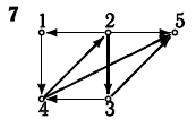
\includegraphics{16_1}
\end{center}

\underline{Решение:}

Построим матрицу смежности данного графа:

$$A=
\begin{pmatrix}
		0 & 0 & 0 & 1 & 0\\
		1 & 0 & 1 & 0 & 1\\
		0 & 0 & 0 & 1 & 1\\
		0 & 1 & 0 & 0 & 1\\
		0 & 0 & 0 & 0 & 0
\end{pmatrix}.$$

Согласно теореме о числе маршрутов длины n их количество находится
как $A^n$. Тогда, число маршрутов длины 2 и 3 и 4 соответственно:

$A^2$=
\begin{pmatrix}
		0 & 1 & 0 & 0 & 1\\
		0 & 0 & 0 & 2 & 1\\
		0 & 1 & 0 & 0 & 1\\
		1 & 0 & 1 & 0 & 1\\
		0 & 0 & 0 & 0 & 0
\end{pmatrix},
$A^3$=
\begin{pmatrix}
		1 & 0 & 1 & 0 & 1\\
		0 & 2 & 0 & 0 & 2\\
		1 & 0 & 1 & 0 & 1\\
		0 & 0 & 0 & 2 & 1\\
		0 & 0 & 0 & 0 & 0
\end{pmatrix},
$A^4$=
\begin{pmatrix}
		0 & 0 & 0 & 2 & 1\\
		2 & 0 & 2 & 0 & 2\\
		0 & 0 & 0 & 2 & 1\\
		0 & 2 & 0 & 0 & 2\\
		0 & 0 & 0 & 0 & 0
\end{pmatrix}.

По матрице $A^2$ найдем число маршрутов длины 2 из вершины № 3 в № 4
– это элемент $a_{34}$, т.е. 0.

Общее число маршрутов длины 3 – это сумма всех элементов матрицы $A^3$
, т.е. 13.

Общее число маршрутов длины 4 – это сумма всех элементов матрицы $A^4$
, т.е. 16.

Ответ: число маршрутов длины 2 из вершины 3 в 4 равно 0, общее число
маршрутов длины 3 – 13, общее число маршрутов длины 4 – 16.

\end{document}
